\section{Critical Slowing Down}
\label{sec:csd}

Critical slowing down and associated early warning signals of critical transitions \cite{schefferCriticalTransitionsNature2009, boettigerEarlyWarningSignals2013, georgeEarlyWarningSignals2021} have been seen in a variety of empirical contexts; in each case, certain detectable statistical trends in a time series appear leading up to a critical transition. A theoretical basis for these leading indicators is rooted in bifurcation theory. 

It should be remarked that another set of indicators for certain critical transitions, not discussed further here, are the spatial pattern-formation mechanisms (e.g. systematic formation of vegetation spots or stripes preceding desertification \cite{dakosSlowingSpatiallyPatterned2011, bastiaansenStablePlanarVegetation2019}). 

%Asymptotic resilience helps determine a bound on the rate of return to equilibrium after a small perturbation to the system. Because local bifurcation is characterized by $Re(\lambda_1)$ passing through zero, recovery typically becomes slower when closer to the verge of bifurcation. This is the core idea of critical slowing down. %, explained further in this section. 

%Roughly, when an ODE approaches a tipping point (specifically, a local bifurcation) where an attracting rest point destabilizes, the rest point gradually loses asymptotic resilience, becoming slower to recover from small perturbations. Since real world systems are naturally perturbed all the time, this loss of asymptotic resilience ought to be empirically observable -- indeed, variance and auto-correlation in the system state tend to increase leading up to tipping. Intuitively speaking, this is because a slow-recovering system stays far away from the mean longer, so variance increases; and because the current state of a slowly moving system tends to stay more similar to its next state, so auto-correlation increases as well (Figure \todo{ref figure}).

%\todo{insert figure}

%Formally, critical slowing down and its associated early warning signals can be explained as in the following subsections. 

%For the purposes of this paper, we will focus on saddle-node (a.k.a fold) %(transcritical and pitchfork?) and Hopf bifurcations, while skipping over much of the preliminary theory. 

\subsection{Local Bifurcation}

For a detailed treatment of local bifurcation theory, see any standard reference. For the purposes of this paper, we include a brief overview focusing mainly on intuitive behavior. 

Consider a parameterized family of ODEs
%
\begin{equation}
	x' = f(x, p)
\end{equation}
%
$f: \mathbb{R}^n \times \mathbb{R} \to \mathbb{R}^n$. Here, $x$ represents state variables, while $p$ represents a parameter. 

%Assume that there is a rest point $f(x_0,p_0) = 0$ for some value of the parameter $p = p_0$. Also suppose the Jacobian $\mathbf{A} = Df(x_0, p_0)$ is hyperbolic.
%%
%%If the Jacobian $\mathbf{A} = Df(x_0, p_0)$ is hyperbolic, then within a neighborhood of $x_0$ the dynamics are topologically conjugate to those of a linear ODE. 
%%
%Because all its eigenvalues are nonzero, $\mathbf{A}$ is an invertible transformation, and the Implicit Function Theorem applies to $f$. This produces a curve $p \to c(p)$ in $\mathbb{R}^n$, defined locally for $p \in [p_0-\epsilon, p_0 + \epsilon]$, such that $c(p_0) = x_0$ and $f(c(p), p) = 0$. 
%
%In other words, if the value of the parameter is adjusted slightly, there will still be a rest point at $c(p)$. Further, since the eigenvalues of $\textbf{A}$ are continuous with respect to $x$ and $p$, that rest point %$(c(p), p)$ for $p$ sufficiently close to $p_0$ 
%is stable if and only if $(x_0,p_0)$ was stable. Thus, the only possible way for a small adjustment in parameter value to lead to a sudden loss of a stable rest point is if $\mathbf{A}$ is non-hyperbolic. Let us focus on that case.
%\todo{move most of the above bifurcation discussion to the appendix or remove it?}

Conceptually, a local bifurcation is a critical state at which a very small change in the parameter value $p$ causes a drastic change in the qualitative nature of a rest point. In particular, its local topology changes -- for example, the rest point could switch between being stable and unstable, or it could disappear altogether. It is well known that such a change in local topology is only possible at non-hyperbolic rest points. 

\begin{definition}
	A \textbf{local bifurcation} occurs at ${\displaystyle (x_{0}, p_{0})}$ if the Jacobian matrix ${\displaystyle {\mathbf{D}f(x_{0},p _{0})}}$ has an eigenvalue with zero real part. Note this could either be a real eigenvalue $\lambda = 0$ or it could be a pair of imaginary eigenvalues $\lambda = \pm \omega i$. In the former case, a \textbf{saddle-node} or \textbf{fold} bifurcation occurs. In the latter, a \textbf{Hopf} bifurcation occurs. \qed
\end{definition}

For simplicity, the term saddle-node bifurcation used here subsumes what are commonly termed transcritical and pitchfork bifurcations, while usage may vary between different authors. However, the distinction between the three categories is useful from an applied point of view, because they reflect different behavior. 

Briefly, a true \textbf{saddle-node/fold bifurcation}, which is neither of the other two types, involves the simultaneous creation or destruction of two equilibria -- it has also been called a ``blue-sky" bifurcation, because two points appear out of or disappear into the blue sky. Saddle-node bifurcations are often catastrophic events whose reversal is difficult or impossible. A prototypical example appears in consumer-resource models (e.g. a population of fish under harvesting pressure). As the consumption/harvesting rate increases, the range of sustainable population sizes shrinks. When the two endpoints of the range collide, the sustainable region disappears, suddenly implying population extinction. 

A \textbf{pitchfork bifurcation}, is similar, but there is already an existing rest point, so that the system switches locally between having one or three rest points; pitchfork bifurcations only occur in sufficiently symmetrical systems, a scenario that does not commonly occur in ecological applications. 

A \textbf{transcritical bifurcation} involves no new birth or death of rest points; instead, a stable and an unstable rest point collide and exchange stabilities with each other. An example occurs in compartmental models of infectious disease transmission. When a parameter known as the basic reproduction number, $R_0$, is increased past a critical value of 1, the disease-free equilibrium destabilizes, bequeathing stability to an endemic equilibrium instead. Transcritical bifurcations tend to be relatively gradual rather than catastrophic transitions -- for instance, for $R_0$ slightly above 1, the new endemic state involves a low prevalence of disease; further, if $R_0$ is decreased back below 1, reign of the disease-free equilibrium is reinstated. 

Finally, a \textbf{Hopf bifurcation} differs from all the others in that a periodic orbit is created or destroyed. As an example, see Figure \ref{fig:predator_prey_reachable_sets}, where an attracting cycle representing oscillating predator and prey populations is born when the parameter $K$ is somewhere between 3 and 4.

%\begin{example}
%	Consider a simple harvesting model $$x' = x(1-x)-h.$$
%	$h$ represents a constant harvesting rate; in the absence of it, the population $x$ undergoes logistic growth to a carrying capacity of 1. As $h$ is gradually increased, the stable population size, $x^{\ast} = \frac{1+\sqrt{1-4h}}{2}$, decreases from 1. 
%	Then, at $h = 1/4$, the system undergoes a saddle-node bifurcation, and the stable equilibrium disappears, implying extinction for the population. (Figure \ref{fig:harvesting_bifurcation_diagram}). 
%	
%	\begin{figure}[ht]
%		\centering
%		\captionsetup{width=0.5\linewidth}
%		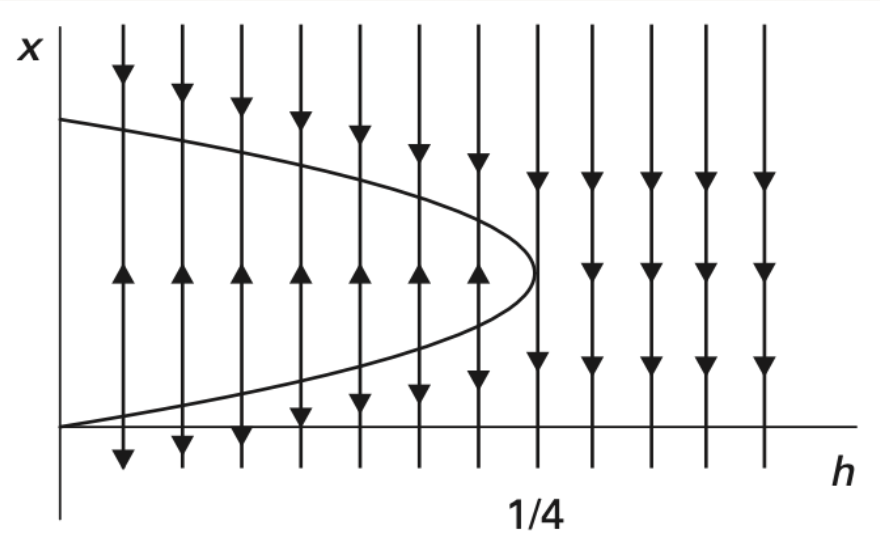
\includegraphics[width=0.5\textwidth]{figs/harvesting_bifurcation_diagram}
%		\caption{Bifurcation diagram for harvesting model $x' = x(1-x)-h$. } 
%		\label{fig:harvesting_bifurcation_diagram}
%	\end{figure} 
%	
%	\todo{cite Hirsch, Smale, Devaney in figure}
%	
%	Computing the dominant (and only) eigenvalue at $x^{\ast}$:
%	\begin{gather}
%		Df(x^{\ast}) = 1-2x^{\ast} = -\sqrt{-1-4h}\\
%		\implies \lambda_1 = -\sqrt{-1-4h}
%	\end{gather} 
%
%	
%\end{example}


%Examples of bifurcation types, normal forms?
%
%Subcritical and supercritical?


\subsection{Critical Slowing Down and Early Warning Signals}

From the previous subsection, we know that local bifurcations are characterized by an eigenvalue's real part approaching and passing through zero. For a stable rest point, all of whose eigenvalues' real parts are negative, this necessarily means it is the dominant eigenvalue's real part which passes through zero. Hence, local bifurcation involving an abrupt change to a steady state is characterized by asymptotic resilience going to zero. We also know that asymptotic resilience provides a bound on long term recovery rates from small perturbations. So, leading up to the bifurcation, recovery rates tend to slow, and this phenomenon is termed critical slowing down. 

Since real world systems frequently face natural perturbations, this slowing down of recovery rate ought to be empirically observable -- indeed, variance and auto-correlation in the system state tend to increase leading up to bifurcation. Intuitively speaking, this is because a slow-recovering system stays far away from the mean longer, so variance increases; and because the current state of a slowly moving system tends to correlate more to its future state, so auto-correlation increases as well (Figure \ref{fig:csd}).

\begin{figure}[ht]
	\centering
	\captionsetup{width=0.9\linewidth}
	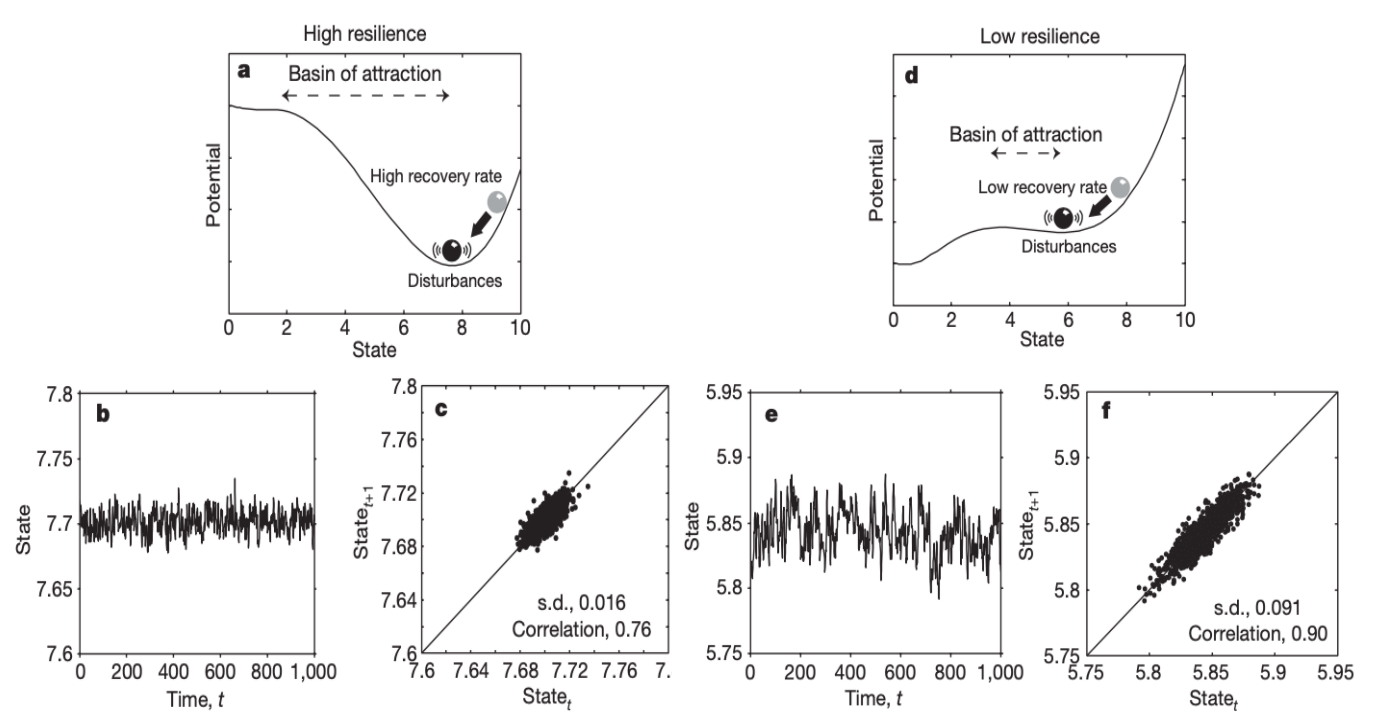
\includegraphics[width=\textwidth]{figs/critical_slowing_down}
	\caption{Critical slowing down and early warning signals. Left: far from bifurcation, high asymptotic resilience, low variance, and low auto-correlation. Right: close to bifurcation, low asymptotic resilience, high variance, and high auto-correlation. Figure reproduced from \cite{schefferEarlywarningSignalsCritical2009a}.}
	
	\label{fig:csd}
\end{figure} 

Formal derivations of the existence of these early warning signals (increased variance and increased auto-correlation) were difficult for me to find in the literature. 
%
An approach has been taken in \cite{schefferCriticalTransitionsNature2009}, approximating the decay by a discrete auto-regressive process with random additive noise applied after each period $\Delta t$,
$$|x_{n+1}-x^{\ast}| = e^{\lambda \Delta t}|x_n-x^{\ast}|+\sigma\epsilon_n.$$
However, it requires the simplifying assumption that return between disturbances is precisely exponential. Another approach has been taken in \cite{ritchieEarlywarningIndicatorsDynamic2016} where the trajectory is modelled as a continuous stochastic mean-reverting process (an Ornstein-Uhlenbeck process), which is the continuous analog of the auto-regressive process of the previously mentioned authors. But this has the same underlying issue of a fundamental simplifying approximation. 

Neubert and Caswell in \cite{neubertAlternativesResilienceMeasuring1997a} emphasize that asymptotic resilience crucially ignores short term behavior. For example, while decay rates are exponential in the limit, perturbations could actually amplify in the short term, and this amplification could happen for arbitrarily small perturbations (see discussion about reactivity at the end of subsection \ref{sec:asymp_res}). As a result, simplifying assumptions like precise exponential decay are not always reasonable assumptions. 

Typically, discussions of early warning indicators are framed from within applied point of view. Empirically, increased variance and increased auto-correlation have indeed been observed in various example systems, and this has often been taken as evidence of their existence in general. Yet, one drawback to the informal treatment is that the precise conditions under which these early warning signals arise, and hence their reliability across different systems and circumstances, remain somewhat unclear. 

%mention flickering and increased skewness?



%\subsection{Limitations}
	
